% Бүлэг 1

\chapter{Хэрэгжүүлэлтын хэсэг}

\label{Chapter3}
\pagecolor{white}

%-------------------------------------------------------------------------------
%	SECTION 1
%-------------------------------------------------------------------------------
\section{Системийн шаардлага}
Систем нь түлхүүр үүсгэх файл хадгалах сервер, өгөгдөл эзэмшигч, өгөгдөл хэрэглэгч гэсэн үндсэн гурван хэсгээс тогтоно. Өгөгдөл эзэмшигч бүртгэл үүсгэж өөрийн нийтийн түлхүүр болон хувийн түлхүүрийг үүсгэж авна.Хувийн түлхүүрийг өөрийн төхөөрөмж дээр авч явах ёстой учир десктоп программ бичих хэрэгтэй болсон. Файл шифрлэх болон тайлах үйлдлийг өөрийн төхөөрөмж дээр үйлдэнэ. Мөн ямар нэг ReKey зэрэг хувийн түлхүүртэй холбоотой үйлдлүүдийг хэрлэгч өөрийн төхөөрөмж дээр хийх ёстой. \\

\textbf{Системийн оролцогч}
\begin{itemize}
    \item Хэрэглэгч
\end{itemize}

\textbf{Системийн тоглогч}
\begin{itemize}
    \item Файл эзэмшигч
    \item Файл хэрэглэгч
\end{itemize}

\subsection*{Функцийн шаардлага}
Файл эзэмшигчийн функционал шаардлага:
\begin{itemize}
    \item Системд өөрийн бүртгэлийг үүсгэх
    \item Файл оруулах, шифрлэх
    \item Файлыг тайлах хэрлэгч сонгох
    \item Шифрлэсэн файлыг хуваалцсан хэрлэгчдийн жагсаалт
\end{itemize}
Файл хэрэглэгчийн функционал шаардлага:
\begin{itemize}
    \item Системд өөрийн бүртгэлийг үүсгэх
    \item Өөрт хуваацлсан файлын жагсаалт
    \item Өөрийн хуваацлсан файлын жагсаалт
    \item Файлыг хэн хэнтэй хуваалцсан жагсаалт
    \item Файлыг татаж авах
    \item Шифрлэсэн файлыг тайлах
\end{itemize}

\subsection*{Функцийн бус шаардлага}
\begin{enumerate}
    \item Файлыг шифрлэх, шифрийг тайлах хурдан гүйцэтгэдэг байх
    \item Хэрэглэгчийн интерфейс ойлгомжтой энгийн байх.
    \item Прокси серверт файлыг шифрлэсэн байдлаар хадгалах, хуваалцах
    \item Өөрийн бүртгэлийг ашиглаж нэвтрэх
    \item Хувийн түлхүүрийг хэрлэгчийн төхөөрөмж дээр авч явах
\end{enumerate}

\subsection*{Юзкейс диаграмм}
Хэрэглэгчид болох файл эзэмшигч болон файл хэрлэгч нь ямар үйлдлүүдийг системд хийж болохыг харуулсан хэрэглээний диаграмм (Зураг \ref{fig:usecase})-т харууллаа.

\begin{figure}[H]
    \centering
    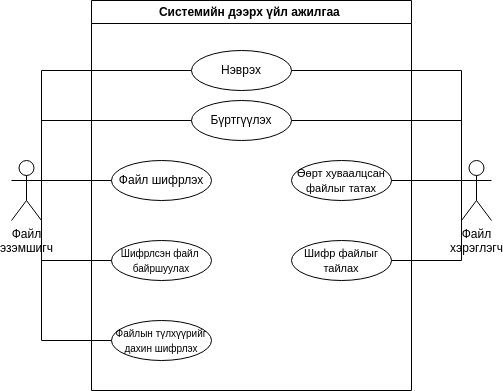
\includegraphics[scale=0.6]{Figures/usecase.drawio.png}
    \caption[Usecase diagram]{Юзкейс диаграмм}
    \label{fig:usecase}
\end{figure}

\subsection*{Юзкейс тодорхойлолт}
\begin{table}[H]
    \label{tab:treatments}
    \footnotesize
    \centering
    \begin{tabularx}{\textwidth}{|>{\hsize=0.3\hsize}X|>{\hsize=0.7\hsize}X|}
        \hline
        \multicolumn{2}{|c|}{Бүртгүүлэх}                                                  \\
        \hline
        ID             & 1                                                                \\
        \hline
        Үндсэн тоглогч & Файл эзэмшигч болон файл хэрэглэгч                               \\
        \hline
        Тодорхойлолт   & Хэрэглэгч шинээр бүртгэл үүсгэх                                  \\
        \hline
        Өмнөх нөхцөл   & Шинэ хэрлэгч байх                                                \\
        \hline
        Үндсэн урсгал  & Хэрэглэгчийн мэдээллийг авч өгөгдлийн санд шинэ хэрэглэгч үүсгэх \\
        \hline
        Дараах нөхцөл  & Хэрэглэгч өөрийн бүртгэлтэй болох нэвтрэх боломжтой болох        \\
        \hline
    \end{tabularx}
    \caption{Бүртгүүлэх юзкейсийн тодорхойлолт}
\end{table}

\begin{table}[H]
    % \label{tab:treatments}
    \footnotesize
    \centering
    \begin{tabularx}{\textwidth}{|>{\hsize=0.3\hsize}X|>{\hsize=0.7\hsize}X|}
        \hline
        \multicolumn{2}{|c|}{Нэвтрэх}                                               \\
        \hline
        ID             & 2                                                          \\
        \hline
        Үндсэн тоглогч & Файл эзэмшигч болон файл хэрэглэгч                         \\
        \hline
        Тодорхойлолт   & Системд нэвтрэх                                            \\
        \hline
        Өмнөх нөхцөл   & Бүргэлтэй хэрлэгч байх                                     \\
        \hline
        Үндсэн урсгал  & Хэрлэгчийн нууц үг бүртгэл таарч байгааг шалган нэвтрүүлэх \\
        \hline
        Дараах нөхцөл  & Бусад хэрэглээ рүү хандах боломжтой болох                  \\
        \hline
    \end{tabularx}
    \caption{Нэвтрэх юзкейсийн тодорхойлолт}
\end{table}

\begin{table}[H]
    % \label{tab:treatments}
    \footnotesize
    \centering
    \begin{tabularx}{\textwidth}{|>{\hsize=0.3\hsize}X|>{\hsize=0.7\hsize}X|}
        \hline
        \multicolumn{2}{|c|}{Файл шифрлэх}                      \\
        \hline
        ID             & 3                                      \\
        \hline
        Үндсэн тоглогч & Файл эзэмшигч                          \\
        \hline
        Тодорхойлолт   & Файл эзэмшигч файлыг шифрлэх           \\
        \hline
        Өмнөх нөхцөл   & Систем нэвтэрсэн байх                  \\
        \hline
        Үндсэн урсгал  &
        \begin{minipage}{\linewidth}
            \begin{itemize}
                \item Файлыг сонгох
                \item Санамсаргүй байдлаар түлхүүр үүсгэх
                \item Файлыг тухайн түлхүүрээр шифрлэх
            \end{itemize}
        \end{minipage}
        \\
        \hline
        Дараах нөхцөл  & Тухайн төхөөрөмж дээр шифрлэгдсэн байх \\
        \hline
    \end{tabularx}
    \caption{Файл шифрлэх юзкейсийн тодорхойлолт}
\end{table}

\begin{table}[H]
    \footnotesize
    \centering
    \begin{tabularx}{\textwidth}{|>{\hsize=0.3\hsize}X|>{\hsize=0.7\hsize}X|}
        \hline
        \multicolumn{2}{|c|}{Шифрлэсэн файл серверт байршуулах}        \\
        \hline
        ID             & 4                                             \\
        \hline
        Үндсэн тоглогч & Файл эзэмшигч                                 \\
        \hline
        Тодорхойлолт   & Шифрлэсэн файлыг серверт хуулна               \\
        \hline
        Өмнөх нөхцөл   & Файлыг шифрэлсэн байх                         \\
        \hline
        Үндсэн урсгал  &
        \begin{minipage}{\linewidth}
            \begin{itemize}
                \item Шифрлэсэн файлыг серверт илгээж
                \item Файлын мэдээллийг өгөгдлийн санд нэмэх
            \end{itemize}
        \end{minipage}
        \\
        \hline
        Дараах нөхцөл  & Файлын талаар мэдээллийг авах боломжтой болох \\
        \hline
    \end{tabularx}
    \caption{Шифрлэсэн файл серверт байршуулах юзкейсийн тодорхойлолт}
\end{table}

\begin{table}[H]
    % \label{tab:treatments}
    \footnotesize
    \centering
    \begin{tabularx}{\textwidth}{|>{\hsize=0.3\hsize}X|>{\hsize=0.7\hsize}X|}
        \hline
        \multicolumn{2}{|c|}{Файл хуваалцах}                                 \\
        \hline
        ID             & 5                                                   \\
        \hline
        Үндсэн тоглогч & Файл эзэмшигч                                       \\
        \hline
        Тодорхойлолт   & Файл эзэмшигч файл хуваалцах хүнийг сонгох          \\
        \hline
        Өмнөх нөхцөл   & Файлыг серверт байршуулсан байх                     \\
        \hline
        Үндсэн урсгал  &
        \begin{minipage}{\linewidth}
            \begin{itemize}
                \item Файл хуваалцах хүний нийтийн түлхүүрийг авах
                \item Дахин шифрлэх түлхүүр үүсгэх
                \item Файлыг дахин шифрлэх
            \end{itemize}
        \end{minipage}
        \\
        \hline
        Дараах нөхцөл  & Шифрлэсэн файлыг төхөөрөмж дээр тайлхад бэлэн болох \\
        \hline
    \end{tabularx}
    \caption{Файл хуваалцах юзкейсийн тодорхойлолт}
\end{table}

\begin{table}[H]
    % \label{tab:treatments}
    \footnotesize
    \centering
    \begin{tabularx}{\textwidth}{|>{\hsize=0.3\hsize}X|>{\hsize=0.7\hsize}X|}
        \hline
        \multicolumn{2}{|c|}{Файл татах}                   \\
        \hline
        ID             & 6                                 \\
        \hline
        Үндсэн тоглогч & Файл хэрэглэгч                    \\
        \hline
        Тодорхойлолт   & Дахин шифрлэсэн файлыг татаж авах \\
        \hline
        Өмнөх нөхцөл   & Файлыг хуваалцсан байх            \\
        \hline
        Үндсэн урсгал  & Файлыг татаж авах                 \\
        \hline
        Дараах нөхцөл  & Файлыг тайлхад бэлэн болох        \\
        \hline
    \end{tabularx}
    \caption{Файл татах юзкейсийн тодорхойлолт}
\end{table}

\begin{table}[H]
    % \label{tab:treatments}
    \footnotesize
    \centering
    \begin{tabularx}{\textwidth}{|>{\hsize=0.3\hsize}X|>{\hsize=0.7\hsize}X|}
        \hline
        \multicolumn{2}{|c|}{Шифрлэсэн файлын тайлах}        \\
        \hline
        ID             & 7                                   \\
        \hline
        Үндсэн тоглогч & Файл хэрэглэгч                      \\
        \hline
        Тодорхойлолт   & Татаж авсан шифрлэсэн файлыг тайлах \\
        \hline
        Өмнөх нөхцөл   & Файлыг хуваалцсан байх              \\
        \hline
        Үндсэн урсгал  &
        \begin{minipage}{\linewidth}
            \begin{itemize}
                \item Файлын түлхүүрийг өөрийн хувийн түлхүүрээр тайлах
                \item Файлын түлхүүрээр файлыг тайлах
            \end{itemize}
        \end{minipage}
        \\
        \hline
        Дараах нөхцөл  & Файлыг унших боломжтой болгох       \\
        \hline
    \end{tabularx}
    \caption{Шифрлэсэн файлын тайлах юзкейсийн тодорхойлолт}
\end{table}

%-------------------------------------------------------------------------------
%	SECTION 2
%-------------------------------------------------------------------------------
\section{Системийн загвар}
Файл хуваалцах үйлчилгээ нь хоёр хэсгээс тогтоно. Хэрэглэгчийн интерфейс нь десктоп программ ба тухайн төхөөрөмж дээр татаж суулгана.
Десктоп программ өөр дээр шифрлэх болон шифрийг тайлах үйлдлийг хийнэ. Сервер хэрэгтэй мэдээллийг хангаж хоёр хэрэглэгчийг холбож өгнө.
\begin{figure}[ht]
    \centering
    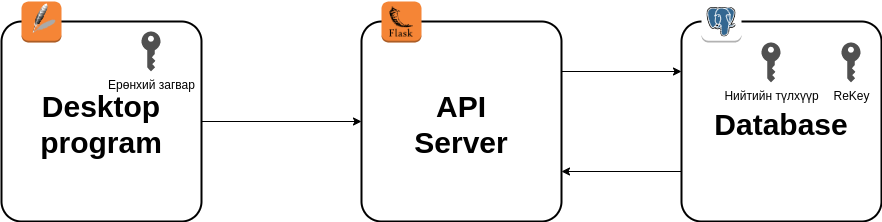
\includegraphics[scale=0.3]{Figures/main_diagram.drawio.png}
    \caption[Usecase diagram]{Ерөнхий загвар}
    \label{fig:main_scheme}
\end{figure}

\subsection*{Үйл ажилгааны диаграмм}
Файл эзэмшигч болон файл хэрэглэгчийн системд нэвтрэхээс файл хуваалцах хүртэл үйл ажиллагааны диаграммыг Зураг \ref{fig:delegatee_diagram} \ref{fig:delegator_diagram}-т харуулав.

\begin{figure}[H]
    \centering
    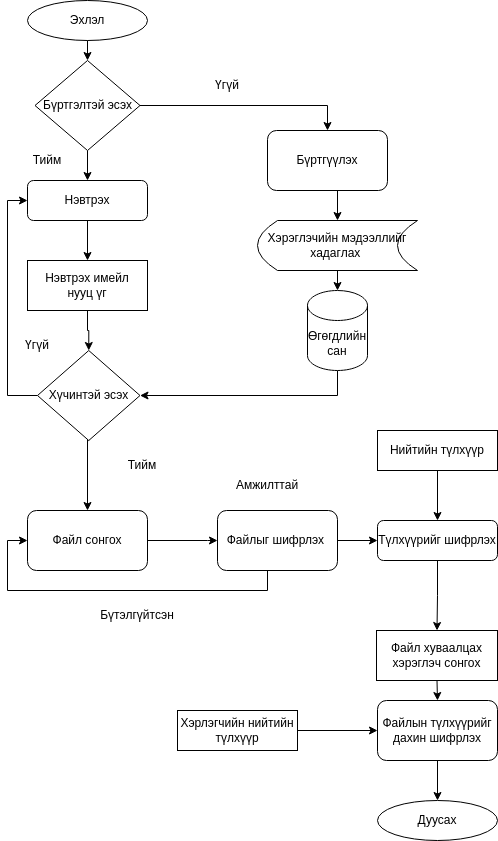
\includegraphics[scale=0.5]{Figures/delegator.drawio.png}
    \caption[pyUmbral]{Файл эзэмшигчийн үйл ажилгааны диаграмм}
    \label{fig:delegator_diagram}
\end{figure}

\begin{figure}[H]
    \centering
    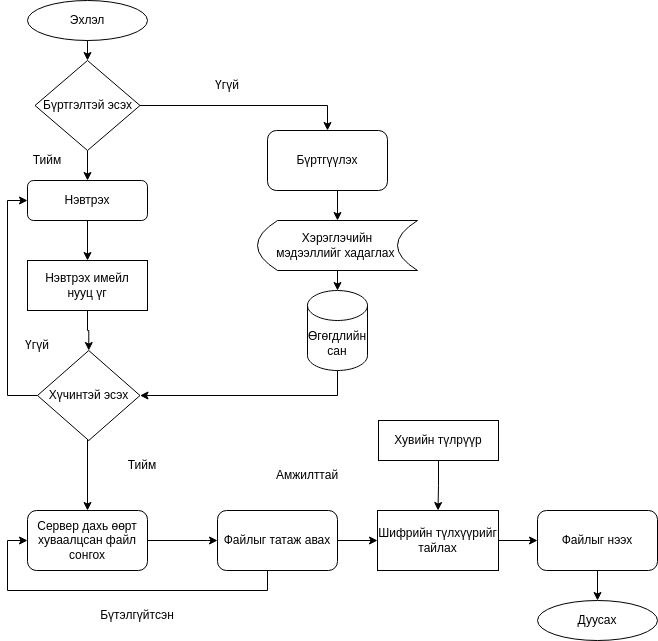
\includegraphics[scale=0.5]{Figures/delegatee.drawio.png}
    \caption[pyUmbral]{Файл хэрэглэгчийн үйл ажилгааны диаграмм}
    \label{fig:delegatee_diagram}
\end{figure}

\subsection*{Өгөгдлийн сангийн бүтэц}
Өгөгдлийн сан нийт дөрвөн хүснэгттэй. Хүснэгт бүрт created\_at, update\_at, deleted\_at гэсэн талбарууд байгаа GORM-аас санаа аван эдгээр талбаруудыг нэмсэн.

\begin{itemize}
    \item \textbf{created\_at} нь тухайн мөр үүсэх үед цагийг бүртгэж авдаг
    \item \textbf{update\_at} нь тухайн мөр өөрчлөгдөх хийх цагийг бүртгэж авдаг
    \item \textbf{deleted\_at} нь тухайн мөрийг устгаагүй байхад хоосон байдаг ба устгасан цагийг бүртгэж авдаг.
\end{itemize}

\begin{figure}[H]
    \centering
    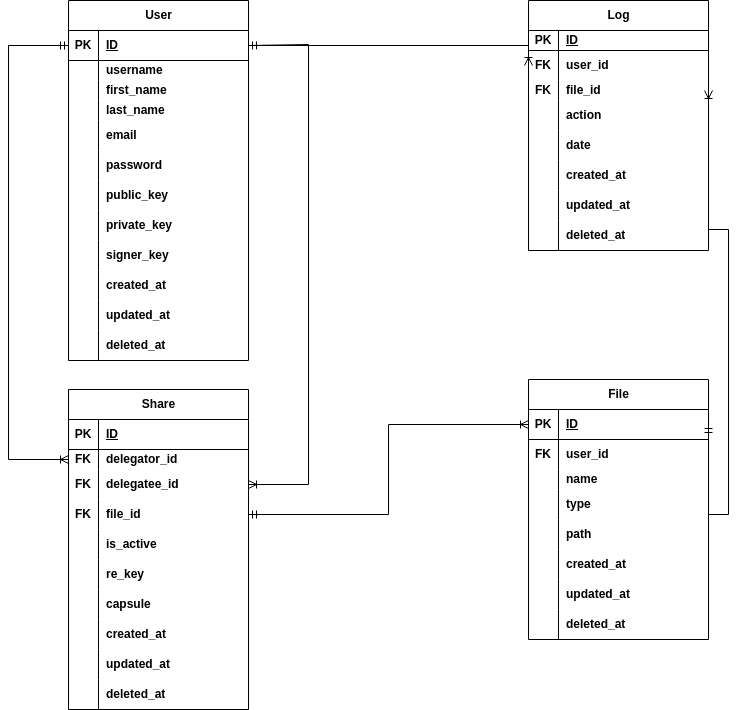
\includegraphics[scale=0.5]{Figures/database.drawio.png}
    \caption[pyUmbral]{Өгөгдлийн сангийн бүтэц}
    \label{fig:database}
\end{figure}

\begin{itemize}
    \item \textbf{User} хэрэглэгчийн хүснэгт. Хэрлэгчийн хувийн түлхүүрийг өгөгдлийн санд хадгалахгүй ба файл хэлбэрээр тухайн төхөөрөмж дээр хадгалж явна.
          \begin{itemize}
              \item ID
              \item username
              \item first\_name
              \item last\_name
              \item email
              \item password
              \item public\_key
              \item signer\_key
          \end{itemize}
    \item \textbf{Share} хүснэгт нь файлыг олон хүнтэй хуваалцах боломжтой болгоно.
          \begin{itemize}
              \item ID
              \item delegator\_id
              \item delagatee\_id
              \item file\_id
              \item is\_active
              \item re\_key
              \item capsule
          \end{itemize}
    \item \textbf{File} Файлын мэдээлэл мөн түлхүүрийг хадгалана.
          \begin{itemize}
              \item user\_id
              \item name
              \item type
              \item path
          \end{itemize}
    \item \textbf{Log} лог хадгалах зориулалтай хүснэгт
          \begin{itemize}
              \item user\_id
              \item file\_id
              \item action
              \item date
          \end{itemize}
\end{itemize}
%-------------------------------------------------------------------------------
%	SECTION 3
%-------------------------------------------------------------------------------
\section{Системийн хөгжүүлэх}

\section*{Хэрэглэгчийн интерфейс}
Хэрэглэгчийн интерфейсийн хувьд зөвхөн дэсктоп программ интерфейстэй байх ба сервер буюу прокси нь ямар нэг график хэрэглэгчийн интерфейс байхгүй зөвхөн API байна.

\begin{figure}[ht]
    \centering
    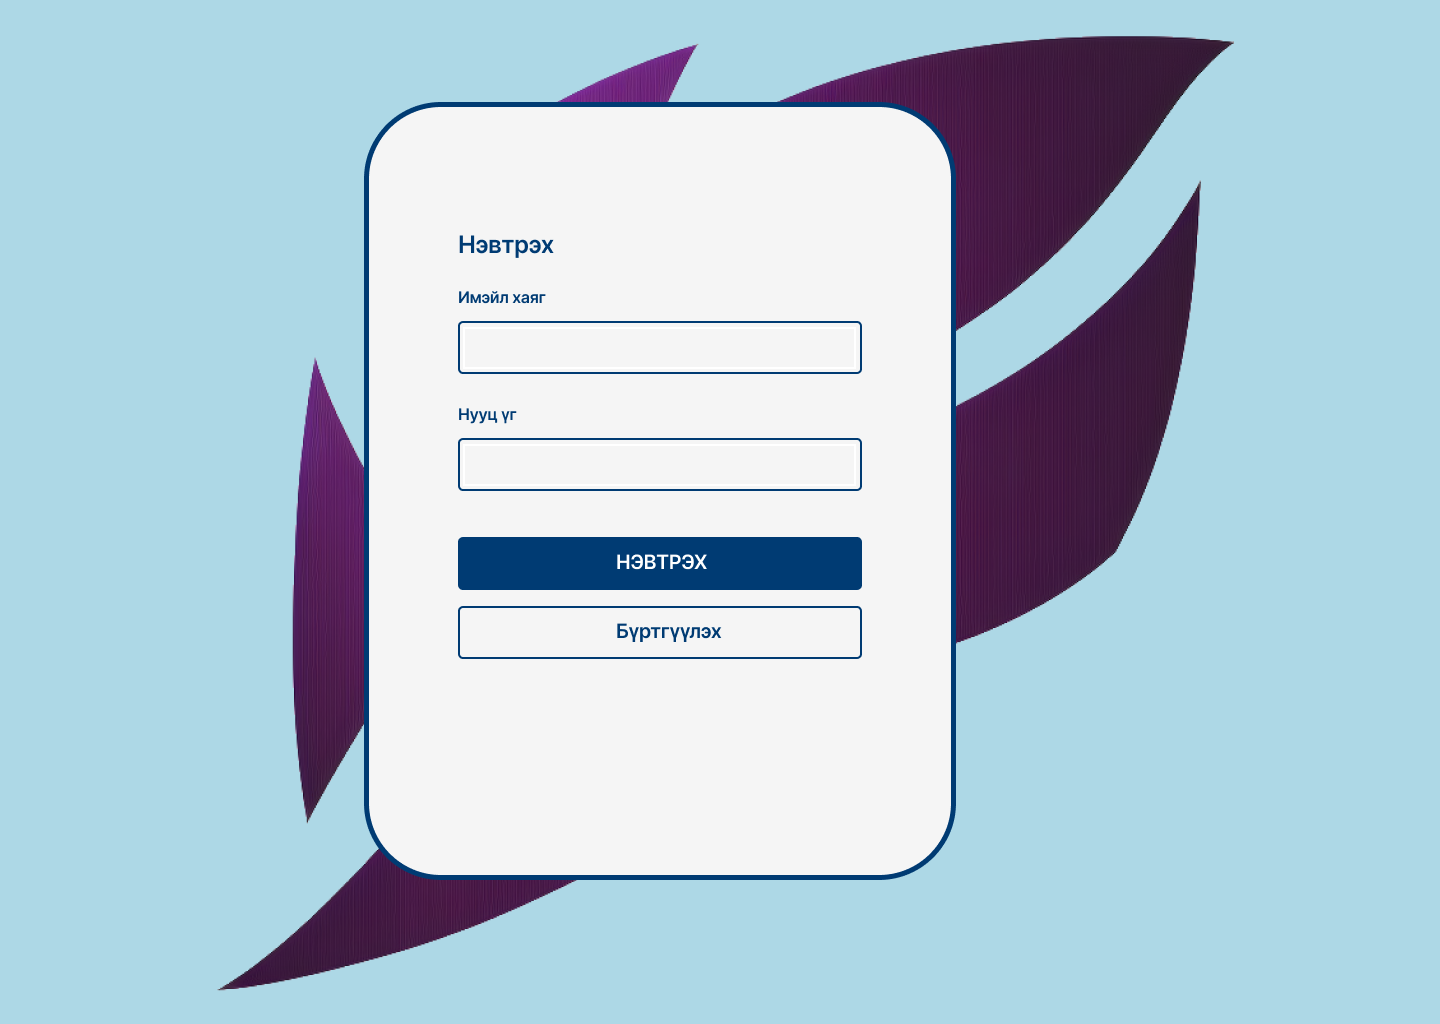
\includegraphics[scale=0.25]{Figures/Login.png}
    \caption[Usecase diagram]{Нэвтрэх цонх}
    \label{fig:login}
\end{figure}

\begin{figure}[ht]
    \centering
    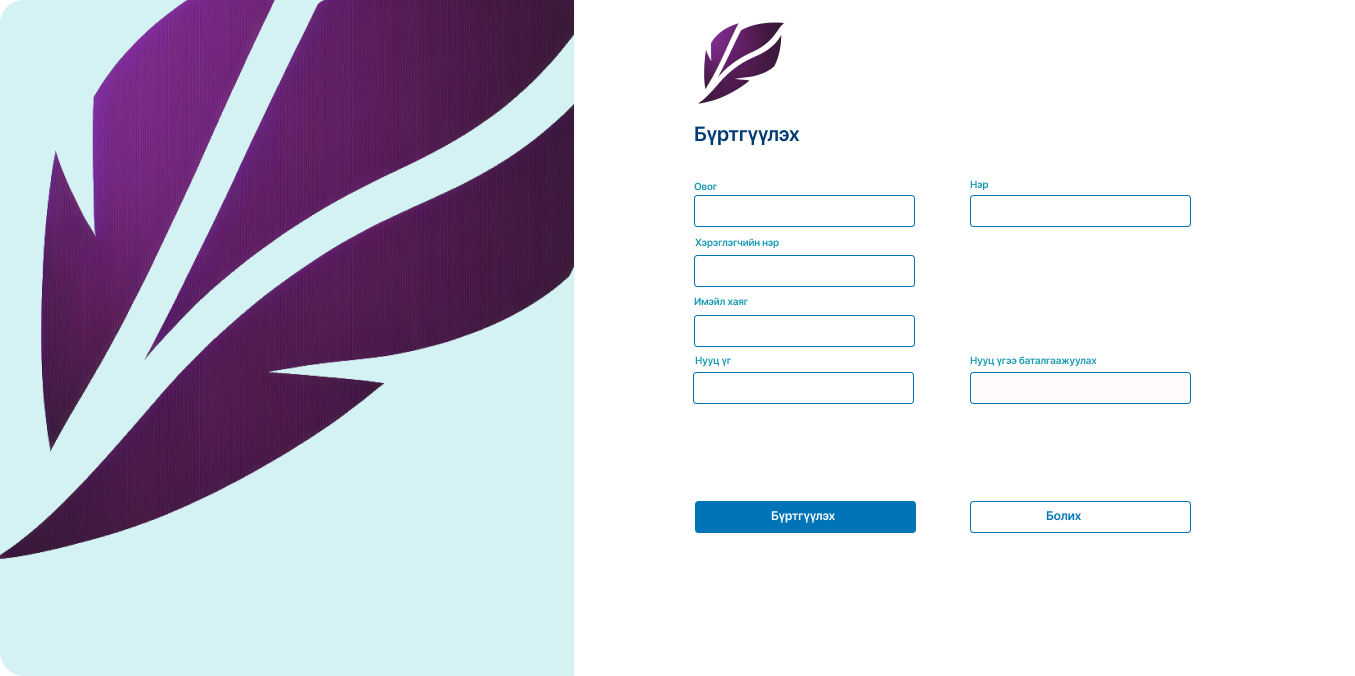
\includegraphics[scale=0.25]{Figures/Register.png}
    \caption[Usecase diagram]{Бүртгүүлэх цонх}
    \label{fig:register}
\end{figure}

\begin{figure}[ht]
    \centering
    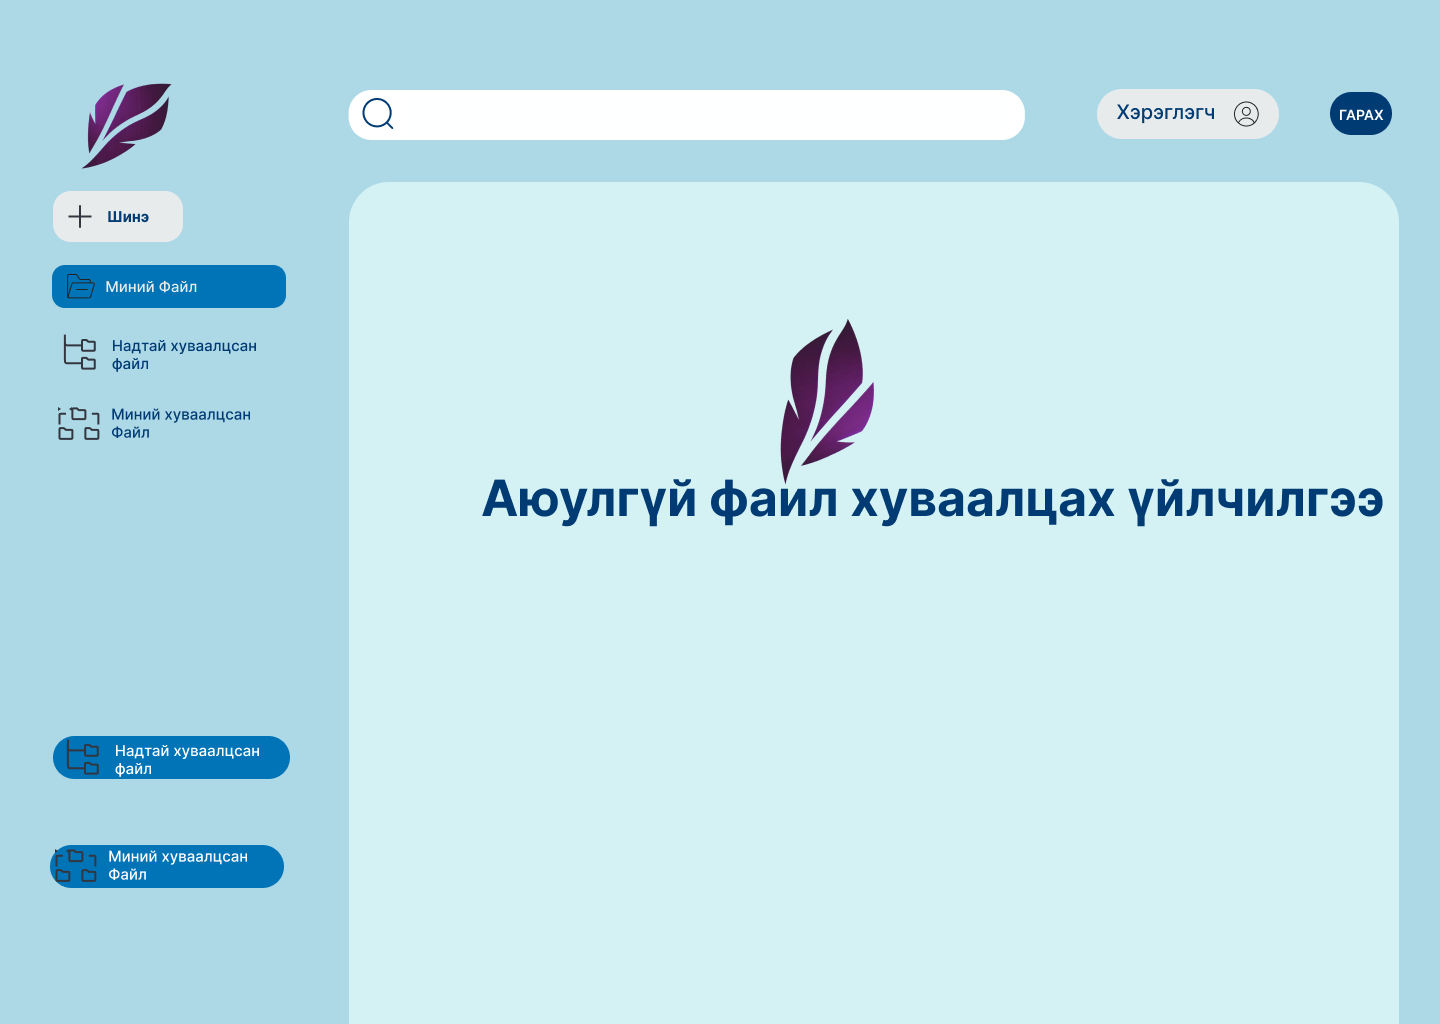
\includegraphics[scale=0.25]{Figures/Main.png}
    \caption[Usecase diagram]{Үндсэн цонх}
    \label{fig:home}
\end{figure}

%-------------------------------------------------------------------------------
%	SECTION 4
%-------------------------------------------------------------------------------
\section{Файл хуваалцах системийг турших}

%-------------------------------------------------------------------------------
%	SECTION 5
%-------------------------------------------------------------------------------

\section{Дүгнэлт}

